%==============================================================================
%  STELAR-improved -- project paper
%  Self-contained single-column preprint style (compiles with pdflatex, no
%  external .cls needed). Build:  pdflatex stelar_improved.tex  (x2 for refs)
%==============================================================================
\documentclass[11pt]{article}

% ---- geometry & fonts -------------------------------------------------------
\usepackage[a4paper,margin=1in]{geometry}
\usepackage[T1]{fontenc}
\usepackage[utf8]{inputenc}
\usepackage{lmodern}
\usepackage{microtype}

% ---- math & symbols ---------------------------------------------------------
\usepackage{amsmath,amssymb,amsfonts}
\usepackage{bm}

% ---- tables, figures, captions ----------------------------------------------
\usepackage{graphicx}
\usepackage{booktabs}
\usepackage{multirow}
\usepackage{array}
\usepackage{caption}
\usepackage{subcaption}
\usepackage{xcolor}

% ---- diagrams ---------------------------------------------------------------
\usepackage{tikz}
\usetikzlibrary{arrows.meta,positioning,fit,backgrounds,calc}

% ---- algorithms -------------------------------------------------------------
\usepackage[ruled,vlined]{algorithm2e}

% ---- references & links -----------------------------------------------------
\usepackage[hidelinks]{hyperref}
\usepackage{cleveref}

% ---- title spacing ----------------------------------------------------------
\usepackage{titlesec}
\titlespacing*{\section}{0pt}{1.4ex plus 1ex minus .2ex}{1ex plus .2ex}
\titlespacing*{\subsection}{0pt}{1.2ex plus 1ex minus .2ex}{0.8ex plus .2ex}

% ---- handy macros -----------------------------------------------------------
\newcommand{\Llat}{\mathcal{L}_{\mathrm{lat}}}
\newcommand{\Lrec}{\mathcal{L}_{\mathrm{rec}}}
\newcommand{\Ltot}{\mathcal{L}_{\mathrm{total}}}
\newcommand{\Etheta}{E_{\theta}}
\newcommand{\Exi}{E_{\xi}}
\newcommand{\Pphi}{P_{\phi}}
\newcommand{\Rpsi}{R_{\psi}}
\newcommand{\wlat}{w_{\mathrm{lat}}}
\newcommand{\wrec}{w_{\mathrm{rec}}}
\definecolor{accent}{RGB}{0,90,160}

% ============================================================================
\title{\textbf{Data Science Project}:\\
 Towards Clinically Robust EEG Foundation Models\\[2pt]
\large Self-Supervised Representation Learning for Neurological Diagnosis}

\author{%
  Mehdi El Kouarati, Alexis Baylet, Amin El Hadri\\[2pt]
  \small Supervisor: Van Tam Nguyen\\
  \small \texttt{}
}
\date{\today}

% ============================================================================
\begin{document}
\maketitle

\begin{abstract}
\noindent
Electroencephalography (EEG) is central to neurological diagnosis and
brain-computer interfaces, yet its low signal-to-noise ratio, non-stationarity
and strong inter-subject variability make general-purpose, transferable
representation learning difficult. Self-supervised EEG \emph{foundation models}
have emerged as a promising answer. This report studies and extends
\textbf{STELAR} (\emph{Spatio-Temporal EEG Latent Alignment \& Reconstruction}),
a compact foundation model whose \emph{dual-space} objective combines patch-level
masked \emph{latent} prediction (semantic stability) with masked \emph{signal}
reconstruction (waveform fidelity), balanced online by a validation-driven
gradient balancer (MTPE-GB). After reviewing the EEG context and the
self-supervised state of the art, we explain the STELAR architecture in detail.
We then describe two targeted improvements we implemented on top of it:
(i)~\textbf{attention-guided masking} that concentrates masking pressure on
semantically salient patches via a teacher-attention prior with a temperature
curriculum, and (ii)~\textbf{asymmetric augmented views} (a clean teacher view
vs.\ a strongly augmented student view) that inject invariance to acquisition
nuisances \emph{without} adding a loss term, plus an optional VICReg anti-collapse
hinge. We report a preliminary, small-scale empirical study (CPU, a 10\% data
slice) validating that all variants train end-to-end without representation
collapse, while finding, as expected at this scale, no measurable separation
between them; isolating their effect requires a larger model, more data, and a
\emph{linear-probing} evaluation. We then report preliminary \emph{downstream}
results (linear probing and fine-tuning) on FACED, TUEV and BCIC-2A (transfer
depends strongly on the adaptation strategy and the classification head), and
outline a domain-adversarial (DANN) extension aimed at reducing subject
overfitting.
\end{abstract}

% ============================================================================
\section{Introduction: the EEG context}
\label{sec:context}

Electroencephalography records the brain's electrical activity from scalp
electrodes at millisecond resolution. It is inexpensive, non-invasive and widely
used for epilepsy monitoring, sleep staging, anomaly detection and
brain-computer interfaces (BCIs). However, EEG is a notoriously difficult signal
for machine learning, for three intertwined reasons:

\begin{itemize}
  \item \textbf{Low signal-to-noise ratio (SNR).} The cortical signal of interest
  is buried under ocular, muscular and line-noise artifacts, as well as
  acquisition-hardware idiosyncrasies. Models that fit the raw signal too closely
  tend to model noise rather than neural content.
  \item \textbf{Non-stationarity.} EEG statistics drift within and across
  recordings (vigilance, electrode drift, impedance changes), so features learned
  on one segment do not trivially transfer to another.
  \item \textbf{Inter-subject variability.} Skull geometry, electrode montage and
  individual neurophysiology differ markedly, so a representation that
  over-specializes to a subject generalizes poorly.
\end{itemize}

Historically, EEG decoding relied on task-specific pipelines (hand-crafted
spectral/spatial features, CSP, Riemannian methods) that work in isolation but do
not scale to general-purpose use. Following the trajectory of NLP and vision, the
field has shifted toward \emph{self-supervised foundation models}: a single
encoder is pre-trained on large unlabeled EEG corpora and then adapted to many
downstream tasks. The central question becomes \emph{which self-supervised
objective yields representations that are both physically faithful and
semantically transferable}, despite the three challenges above. This report
studies a recent, parameter-efficient answer to that question, STELAR, and a
set of targeted improvements to it.

\paragraph{Scope and contributions of this report.} We (i) situate EEG
self-supervised learning and motivate the choice of STELAR
(\Cref{sec:related}); (ii) explain the STELAR architecture and its dual-space
objective in detail (\Cref{sec:stelar}); (iii) present and motivate two
improvements we implemented, attention-guided masking and asymmetric augmented
views, with an optional anti-collapse term (\Cref{sec:improvements}); (iv) report
a preliminary small-scale empirical study of these variants
(\Cref{sec:experiments}); (v) explore architectural directions for the backbone
(\Cref{sec:arch-explore}); and (vi) report preliminary downstream results
(linear probing, fine-tuning, and a domain-adversarial extension) on several
EEG tasks (\Cref{sec:downstream}).

% ============================================================================
\section{Background and state of the art}
\label{sec:related}

\subsection{Self-supervised learning for EEG}
Self-supervised learning (SSL) for EEG has converged on three broad paradigms.

\paragraph{(i) Generative masked modeling.} A portion of the input is masked and
the model reconstructs it in \emph{signal space}. BENDR
adapted masked modeling to EEG; LaBraM refined it with a
neural tokenizer and discretized targets; CBraMod uses
criss-cross attention to capture spatio-temporal structure; and
CSBrain adds cross-scale tokenization and structured sparse
attention. These methods capture local dependencies well but tend to
\emph{over-index on low-level noise and acquisition artifacts}, which can hurt the
high-level abstractions needed for transfer.

\paragraph{(ii) Discriminative / alignment objectives.} These learn invariant
representations by aligning views in a \emph{latent space}, e.g.\ contrastive
methods and, more recently, masked
\emph{latent} prediction such as EEG2Rep. Aligning
masked segments to their own latent targets bypasses raw-signal SNR and removes
the need for curated negatives, but, without an anchor, latent SSL is prone to
\emph{representation collapse}, where the encoder maps everything to a constant.

\paragraph{(iii) Hybrid schemes.} Recent models combine objectives. EEGPT
pairs a momentum teacher for latent matching with signal reconstruction;
EEG-X uses noise-aware masking in raw and latent spaces.
Two recurring weaknesses remain: \emph{coarse-grained supervision} (alignment at a
summary-token level overlooks fine spatio-temporal events), and \emph{optimization
bottlenecks} (fixed loss weights require expensive manual tuning and cannot track
the shifting convergence rates of the constituent tasks).

\subsection{The chosen model: STELAR}
STELAR~\cite{stelar2026,stelarfull} directly targets the two weaknesses above.
It \emph{decouples} representation learning (masked \emph{latent} prediction at the
\textbf{patch level}) from physical grounding (masked \emph{signal}
reconstruction), and \emph{balances} them with a near-zero-overhead, validation-
driven gradient balancer (MTPE-GB) instead of fixed weights. Two properties make
it an attractive base for a project on improving EEG representation learning:

\begin{itemize}
  \item \textbf{Strong linear-probing performance at a tiny size.} STELAR reports
  state-of-the-art \emph{linear-probe} results on most metrics across seven EEG
  benchmarks with only \(\sim\!0.26\)M parameters (\(\sim\!0.11\)M in the encoder),
  versus 4-76M for EEGPT, LaBraM, CBraMod and CSBrain (\Cref{tab:efficiency}).
  Linear probing isolates intrinsic representation quality, so these gains are a
  clean signal that the dual-space objective works.
  \item \textbf{A clear, modular objective.} The two losses and the balancer are
  conceptually separable, which makes the model an ideal substrate for targeted,
  ablation-friendly improvements, exactly what this project needs.
\end{itemize}

\begin{table}[t]
\centering
\caption{Pre-training compute footprint reported by STELAR and baselines.
STELAR reaches SOTA linear probing at a fraction of the size.}
\label{tab:efficiency}
\small
\begin{tabular}{lrrr}
\toprule
Method & Total params & Encoder params & MFLOPs/step \\
\midrule
LaBraM   & 5.99M & 5.8M  & 2{,}583 \\
EEGPT    & 76M   & 25M   & 25{,}000 \\
CBraMod  & 3.95M & 3.9M  & 16{,}679 \\
CSBrain  & 8.90M & 8.9M  & 30{,}913 \\
\textbf{STELAR} & \textbf{0.263M} & \textbf{0.112M} & \textbf{635} \\
\bottomrule
\end{tabular}
\end{table}

% ============================================================================
\section{The STELAR architecture}
\label{sec:stelar}

\subsection{Overview}
STELAR is a teacher-student, dual-space masked predictor (\Cref{fig:arch}). The
input EEG \(S \in \mathbb{R}^{C\times T}\) (\(C=19\) channels, \(T\) samples) is
segmented into non-overlapping 1-second patches and embedded. A 50\% random mask
splits patches into \emph{visible} and \emph{masked}. Four components cooperate:

\begin{enumerate}
  \item \textbf{Online encoder \(\Etheta\)} encodes only the \emph{visible}
  patches.
  \item \textbf{Target encoder \(\Exi\)} (an exponential-moving-average, or EMA,
  copy of \(\Etheta\); no gradient) encodes the \emph{full} unmasked signal to
  produce stable semantic \emph{targets}.
  \item \textbf{Predictor \(\Pphi\)} (one lightweight Transformer layer) predicts
  the latent representations of the masked patches from the visible context.
  \item \textbf{Reconstructor \(\Rpsi\)} (one layer) reconstructs the raw waveform
  of the masked patches, acting as a fidelity regularizer.
\end{enumerate}

\begin{figure}[t]
\centering
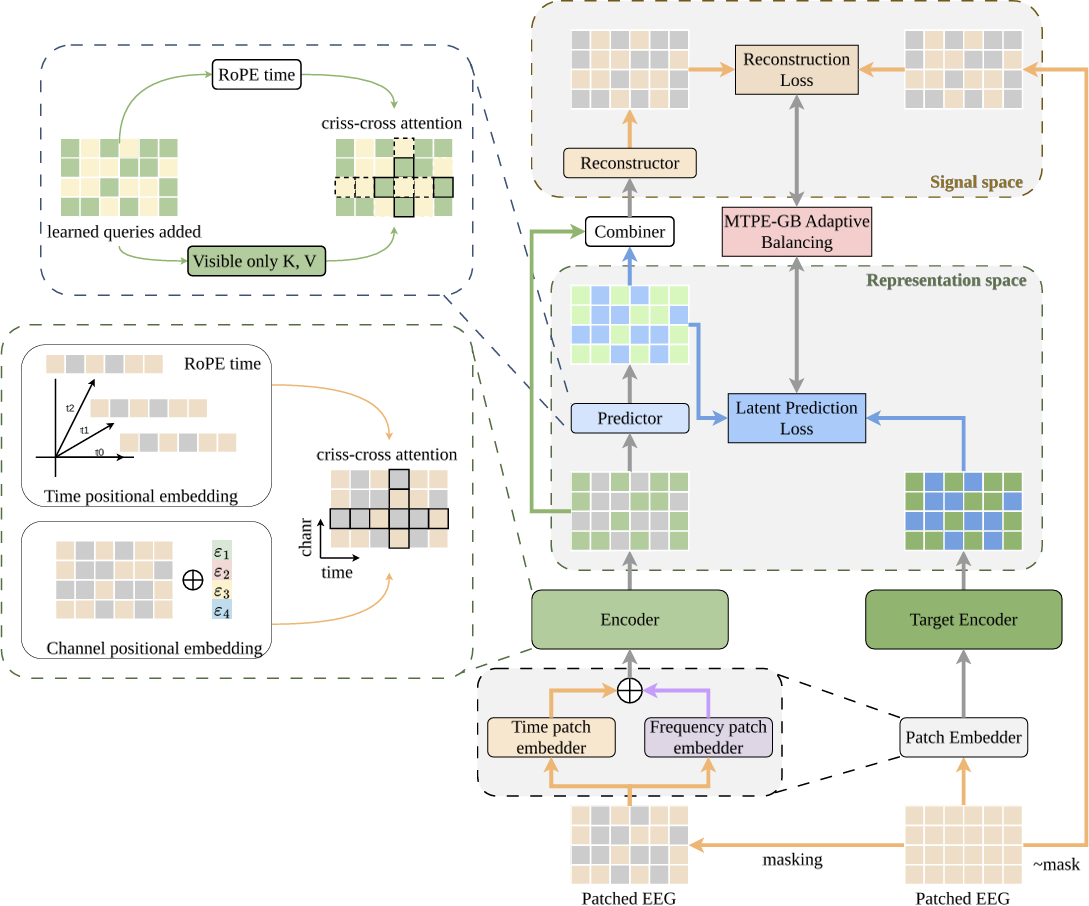
\includegraphics[width=\textwidth]{stelar_arch_fig.png}
\caption{Schematic of the STELAR framework: teacher-guided patch-level masked
latent prediction supervised by a target encoder (EMA updated); lightweight
masked signal reconstruction as a fidelity regularizer; and validation-driven
adaptive balancing between objectives.}
\label{fig:arch}
\end{figure}

\subsection{Patch embedding and encoder backbone}
\paragraph{Dual-branch embedder.} Each patch is embedded by \emph{two} branches in
parallel: a \emph{temporal} branch (1-D convolutions over the raw samples) and a
\emph{frequency} branch (an FFT followed by an MLP). Fusing morphological and
oscillatory cues is important for EEG, whose information lives both in transient
waveforms and in band power.

\paragraph{Criss-Cross encoder.} Modeling full spatio-temporal attention over
\(C\times N\) tokens is expensive. STELAR uses \emph{Criss-Cross
attention}, which factorizes attention into two cheaper
orthogonal passes, across channels (spatial) and across time (temporal),
preserving spatio-temporal context at much lower cost. Positional information is
injected by \emph{Rotary Positional Embeddings} (RoPE) along time and by
\emph{learnable channel embeddings}, so the model is aware of \emph{when} and
\emph{on which electrode} each token sits, and tolerates varying montages.

\subsection{Dual-space objective}
STELAR minimizes a weighted sum of two complementary losses:
\begin{equation}
\Ltot \;=\; \wlat \,\Llat \;+\; \wrec \,\Lrec .
\label{eq:dual}
\end{equation}
\(\Llat\) (masked \emph{latent} prediction) regresses the predicted latents of
masked patches onto their EMA-teacher targets, forcing \emph{semantic
abstraction} and preventing trivial low-level shortcuts. \(\Lrec\) (masked
\emph{signal} reconstruction) recovers the raw waveform of masked patches, acting
as a \emph{fidelity regularizer} that anchors the latent space and helps prevent
dimensional collapse. The two pull in different directions, semantics vs.\
fidelity, which is precisely why their relative weight matters.

\paragraph{Does the latent branch earn its complexity?} It is worth stressing
that the dual-space premise is not self-evident. A recent benchmark of EEG
foundation models, Yang et al.~\cite{yang2026eegfm}, shows that a plain masked
auto-encoder on raw signal (essentially the \(\wlat\!\to\!0\) corner of
\Cref{eq:dual}) can, at sufficient scale, match or surpass far more elaborate
objectives, directly questioning whether a separate latent-prediction branch is
needed at all. STELAR's \(\wlat,\wrec\) extremes therefore double as a built-in
test of this claim: comparing the reconstruction-only (\(\wrec\!=\!1\)) and
latent-only (\(\wlat\!=\!1\)) corners against the balanced objective measures
exactly how much the latent branch adds. We caution, however, that Yang et
al.\ establish their result at \emph{large} scale with full fine-tuning, whereas
our study runs at \(\sim\!2\)\,GB with a tiny model under linear-probe-style
evaluation; at that scale neither corner is expected to separate, which is itself
consistent with their findings that linear probing stays weak and that no clear
scaling law holds.

\subsection{Balancing the objectives: MTPE-GB}
Naively fixing \(\wlat,\wrec\) is brittle: the ``easier'' reconstruction task
tends to dominate the gradient early, and the right balance shifts during
training. Classical gradient-balancing methods (GradNorm,
multi-objective optimization, gradient
surgery) require second-order terms, stored per-task gradient
vectors, or multiple backward passes, prohibitive at scale. STELAR introduces
the \emph{Multi-Task Pre-training EEG Gradient Balancer} (MTPE-GB,
\Cref{alg:mtpegb}): it reweights tasks using only the \emph{scalar validation
losses} already available in the loop, measuring each task's relative
\emph{progress} (current vs.\ initial validation loss) and giving more weight to
the task that is improving more slowly. The overhead is negligible and no manual
tuning is needed.

\begin{algorithm}[t]
\caption{MTPE-GB: validation-driven task balancing}
\label{alg:mtpegb}
\KwIn{model $\Theta$; $k$ tasks; $M$ updates; smoothing $c\in[0,1]$}
Initialize $w_i(0)=1/k$; record initial validation losses $\mathcal{L}^{V}_i(0)$\;
\For{$t=1$ \KwTo $M$}{
  Train one epoch; validate to get current losses $\mathcal{L}^{V}_i(t)$\;
  Progress: $u_i(t) = \big(\mathcal{L}^{V}_i(0) - \mathcal{L}^{V}_i(t)\big)\big/\mathcal{L}^{V}_i(0)$\;
  Raw weights: $\overline{w_i}(t{+}1) = \dfrac{u_i^{-1}(t)}{\sum_{j=1}^{k} u_j^{-1}(t)}$ \quad s.t. $\textstyle\sum_i \overline{w_i}=1$\;
  Smooth: $w_i(t{+}1) \leftarrow c\,\overline{w_i}(t{+}1) + (1-c)\,w_i(t)$\;
}
\end{algorithm}

\subsection{Pre-training setup (reference)}
STELAR is pre-trained on a curated 500-hour subset of TUEG
(0.3-75\,Hz band-pass, 60\,Hz notch, 200\,Hz resample, 30\,s windows, 19
channels, 50\% masking) for 30 epochs with AdamW, peak learning rate
\(10^{-4}\) (warmup + cosine), batch size 64, on A100 GPUs.
\Cref{tab:hparams} summarizes the configuration.

\begin{table}[t]
\centering
\caption{STELAR reference hyperparameters (condensed).}
\label{tab:hparams}
\small
\begin{tabular}{lll}
\toprule
Block & Hyperparameter & Value \\
\midrule
\multirow{4}{*}{EEG sample}
  & Channels / rate & 19 / 200\,Hz \\
  & Window & 30\,s (6000 samples) \\
  & Patch / sequence & 200 (1\,s) / 30 patches \\
  & Mask ratio & 50\% \\
\midrule
\multirow{3}{*}{Encoder}
  & Depth / hidden / heads & 2 / 64 / 2 \\
  & MLP ratio / attention & 4.0 / Criss-Cross \\
  & Position & RoPE(time) + channel emb. \\
\midrule
Predictor & Depth / KV / attention & 1 / global visible-only / Criss-Cross \\
Reconstructor & Depth / attention & 1 / full \\
Teacher & EMA momentum & cosine $0.996 \to 1$ \\
\midrule
\multirow{4}{*}{Pre-training}
  & Epochs / batch & 30 / 64 \\
  & Optimizer / LR & AdamW / $10^{-4}$ (warmup+cosine) \\
  & Weight decay & $10^{-4}$ (cosine) \\
  & Grad clip & 1.0 \\
\bottomrule
\end{tabular}
\end{table}

% ============================================================================
\section{Our project: attempted improvements}
\label{sec:improvements}

Our extensions keep the STELAR backbone, objective and balancer \emph{unchanged}
and intervene only on two axes: \emph{where} masking pressure is applied (\#1) and
\emph{what} the encoder sees (\#2). Crucially, neither adds a loss term, so
MTPE-GB stays a two-task balancer; an optional anti-collapse term (VICReg) can be
switched on as a third task if needed. All variants are exposed as named presets
(\Cref{tab:presets}).

\begin{table}[t]
\centering
\caption{Improvement presets implemented on top of STELAR.}
\label{tab:presets}
\small
\begin{tabular}{lcccl}
\toprule
Preset & \#1 attn-mask & \#2 aug. & VICReg & Role \\
\midrule
\texttt{v0\_baseline} & --- & --- & --- & faithful STELAR reference \\
\texttt{v1\_attnmask} & \checkmark & --- & --- & \#1 isolated (diagnostic) \\
\texttt{v2\_aug}      & --- & \checkmark & --- & \#2 isolated (Option B) \\
\texttt{vA\_combo}    & \checkmark & \checkmark & --- & \#1\,+\,\#2 (Option A) \\
\bottomrule
\end{tabular}
\end{table}

\subsection{Improvement \#1: attention-guided masking}
\paragraph{Idea.} In STELAR, the 50\% mask is random. We instead bias the mask
toward \emph{semantically salient} patches, estimated from the attention
\emph{received} in the last block of the teacher (which already runs a full
forward to produce targets). The intuition is that masking informative regions
makes the prediction task harder and richer than masking arbitrary ones.

\paragraph{Why teacher attention and not signal variance.} Variance conflates
semantics with subject idiosyncrasy; masking by variance would push the encoder
toward subject-specific signatures and hurt generalization. Attention received is
a cleaner semantic-saliency proxy.

\paragraph{Mechanics.} We combine the two Criss-Cross attention maps (spatial and
temporal), each min-max normalized, into an importance map over patches (gradient
detached, it is a sampling prior, not a trained signal). We then sample the mask
via \emph{Gumbel-top-\(k\)} with temperature \(\tau\):
\begin{equation}
\text{perturbed} = \log(\text{importance}) + \tau\cdot\text{Gumbel}, \qquad
\text{mask} = \text{top-}k(\text{perturbed}).
\end{equation}
High \(\tau\) makes noise dominate (\(\approx\) uniform random masking); low
\(\tau\) concentrates on salient patches. A \emph{cosine curriculum} decays
\(\tau\) from \(\tau_{\text{start}}{=}1.0\) to a non-zero floor
\(\tau_{\text{min}}{=}0.1\) over \(\sim\!15\) epochs, so training starts easy and
gradually focuses. Importance is extracted by non-invasive forward-hooks on the
teacher's last block, and the method \emph{falls back to uniform masking} on any
failure (missing modules, shape surprise, NaNs), so it degrades gracefully.

\subsection{Improvement \#2: asymmetric augmented views}
\paragraph{Idea (data2vec-like asymmetry).} The teacher encodes a \emph{weak /
clean} view (stable, clean latent targets), while the student encodes a
\emph{strong-augmented + masked} view and must predict the clean targets.
Invariance to acquisition nuisances then emerges \emph{inside} \(\Llat\), with
\textbf{no extra loss term} (MTPE-GB stays two-task).

\paragraph{Augmentations (raw signal space).} Augmentations are applied to the
model input \emph{before} the patch embedder, so that \emph{both} the convolution
(time) and FFT (frequency) branches see them. The student menu uses moderate
amplitudes appropriate for low-SNR EEG: per-channel amplitude scaling
\(\sim\mathcal{U}(0.8,1.2)\), additive noise, temporal jitter, crop-resize, and
channel-dropout (\(\le\!20\%\), zeroed in the \emph{raw} signal). We deliberately
\emph{exclude} label-/montage-destroying transforms (time-reversal, sign-flip,
channel permutation) and keep \emph{band-dropout off} by default (it harms
band-specific tasks and the FFT branch). Reconstruction and latent targets are
always computed on the \emph{clean} signal.

\subsection{Optional VICReg anti-collapse term}
Stacking strong augmentation (\#2) and hard masking (\#1) raises the risk of
\emph{representation collapse}. Following standard practice, we always
\emph{log} the per-dimension embedding standard deviation of both teacher and
student; if it collapses, an optional VICReg \emph{variance hinge} on the
\emph{student} embeddings (which carry gradient) can be enabled as MTPE-GB's third
task. Covariance/invariance VICReg terms are intentionally omitted: invariance is
already provided by \(\Llat\), and the variance hinge alone is the cheap
anti-collapse guard.

\subsection{Decision protocol}
Additivity of \#1 and \#2 is a hypothesis, not a guarantee, so we follow an
empirics-first protocol: run \#1-alone and \#2-alone with identical
seeds/splits; if \#1-alone barely helps, do \emph{not} combine and ship Option~B
(\#2); if both clearly help, combine into Option~A and tune \emph{sequentially}
(fix \#2 at moderate defaults, search \#1's \(\tau\) schedule, then lightly
retouch \#2), never jointly.

% ============================================================================
\section{Preliminary empirical study}
\label{sec:experiments}

\paragraph{Goal.} Before any large-scale comparison, we validated that the three
model scripts (\texttt{v0\_baseline}, \texttt{v1\_attnmask}, \texttt{v2\_aug})
train end-to-end and behave sanely. This is a \emph{smoke-scale} study, not a
performance benchmark.

\paragraph{Setup.} We trained on a single LMDB (a 10\% validation slice of the
pre-processed TUEG pipeline: 4{,}674 windows of shape \([19,30,200]\), i.e.\
only \(\sim\!2\)\,GB of data), split \(90/10\) into train/validation \emph{on the
fly}. All three presets, the baseline \emph{and} both proposed improvements
(\texttt{v1\_attnmask}, \texttt{v2\_aug}), were trained on this same slice, with
the \texttt{tiny} configuration (encoder hidden 64, depth 2; \(\sim\!304\)K total
parameters), batch size 64, 30 epochs, seed 7, learning rate \(10^{-4}\). Only the
preset changed between runs. This very small scale was \emph{forced by GPU
limitations}, not chosen: runs were executed on whatever compute was available at
the time (CPU or a small GPU, depending on the run), which is why we could not
pre-train the improvements on anything larger than this \(\sim\!2\)\,GB slice.

\paragraph{Results.} \Cref{tab:results} reports validation metrics. The three
variants behave almost identically. In all of them the \emph{latent} alignment
loss falls from \(\approx\!1.0\) to \(\approx\!0.04\) (the student matches the EMA
teacher well), the \emph{reconstruction} loss plateaus near \(0.996\) (the tiny
MLP reconstructor saturates at this scale), and the embedding standard deviation
contracts from \(\approx\!0.87\) to \(\approx\!0.20\) but \emph{stays clearly
positive}, i.e.\ \textbf{no collapse}. The attention curriculum of \#1 anneals
as designed (\(\tau:1.0\!\to\!0.1\)). The best total validation loss differs by
only \(\sim\!0.2\%\) across presets, which is within noise.

\begin{table}[t]
\centering
\caption{Preliminary validation metrics (30 epochs, CPU, 10\% data slice, single
seed). Differences across presets are within noise; this run validates the
pipeline, not the relative merit of the improvements.}
\label{tab:results}
\small
\begin{tabular}{lccc}
\toprule
Metric (validation) & \texttt{v0\_baseline} & \texttt{v1\_attnmask} & \texttt{v2\_aug} \\
\midrule
Best total loss (epoch)      & 0.7428 (ep5) & 0.7413 (ep4) & \textbf{0.7410} (ep4) \\
Final total loss (ep29)      & 0.8116 & 0.8120 & 0.8114 \\
Latent loss (first $\to$ last) & 0.998 $\to$ 0.042 & 0.995 $\to$ \textbf{0.038} & 0.998 $\to$ 0.040 \\
Recon loss (first $\to$ last)  & 1.293 $\to$ 0.996 & 1.292 $\to$ 0.996 & 1.293 $\to$ 0.996 \\
Student emb.\ std (first $\to$ last) & 0.894 $\to$ 0.243 & 0.893 $\to$ 0.236 & 0.883 $\to$ 0.228 \\
Teacher emb.\ std (first $\to$ last) & 0.869 $\to$ 0.198 & 0.869 $\to$ 0.191 & 0.869 $\to$ 0.194 \\
Collapse & none & none & none \\
\bottomrule
\end{tabular}
\end{table}

\paragraph{Reading the loss dynamics.} The total loss \emph{rises} after epoch
4-5 and then plateaus; this is \emph{not} a regression. As the latent loss
collapses toward zero, MTPE-GB shifts weight toward reconstruction
(\(\wrec:0.50\!\to\!0.81\)); the weighted sum therefore increases even though both
individual losses are flat or still decreasing. This is exactly the adaptive
behavior MTPE-GB is designed to produce.

\paragraph{Interpretation.} All three pipelines train cleanly, converge, and show
no collapse, so the engineering is validated. However, \#1 and \#2 show \emph{no
measurable advantage} over the baseline here. This is expected: a \texttt{tiny}
model on a 10\% data slice for 30 CPU epochs is far too small a regime for these
improvements to express themselves, and the dominant dynamics (latent loss
\(\to 0\), reconstruction plateau, MTPE-GB reweighting) swamp any subtle effect.
Consistent with the decision protocol, the empirics at this scale say
``no signal yet'' rather than picking a winner.

\paragraph{Threats to validity.} Single seed, limited compute (CPU / a small
GPU), a small \(\sim\!2\)\,GB in-distribution slice (measuring fit, not transfer),
and a tiny model. None of these allow conclusions about the improvements' true
effect; they only establish correctness and stability.

% ============================================================================
\section{Project organization: two complementary axes}
\label{sec:axes}

Beyond the objective-level improvements of \Cref{sec:improvements}, our project
work was organized around two further axes. Foundation models aim to learn
\emph{general} EEG representations that can be reused across many downstream
tasks: instead of training a model from scratch for every dataset, the encoder is
pre-trained on large, diverse data and then adapted by fine-tuning. This is
especially relevant for EEG, where labeled data are limited, noisy and highly
variable across subjects, devices, protocols and montages. Because EEG is
high-dimensional, non-stationary and strongly subject-dependent, adapting such a
model is not only a matter of fine-tuning the final classifier, but also of
reconsidering the backbone, temporal patches, channels, positional information
and inter-subject variability. Accordingly, the first axis
(\Cref{sec:arch-explore}) studies modifications to the STELAR \emph{backbone}, and
the second (\Cref{sec:downstream}) studies \emph{downstream} fine-tuning and
evaluation.

% ============================================================================
\section{Axis 1: architectural exploration of STELAR}
\label{sec:arch-explore}

The first axis reconsiders \emph{how a foundation model should represent an EEG
signal}, rather than merely tuning hyperparameters. EEG has a particular
structure: a temporal axis, cut into patches, and a channel axis corresponding to
electrodes on the scalp. Channels are therefore not independent dimensions
(they also carry \emph{spatial} information), which is why the choices around
temporal patches, channel embedding, positional encoding and attention matter.

We considered two main directions. The first concerns \emph{channel information}:
whether the model should learn a representation specific to each channel, or
instead be given more flexibility to adapt to different EEG montages. The second
concerns \emph{positional encoding}: the model must retain a notion of position in
time, but potentially also a notion of spatial structure between electrodes.
These directions both motivate the architectural choices already present in STELAR
(learnable channel embeddings, RoPE in time) and frame possible extensions toward
montage-agnostic and spatially-aware encoders. A recent example of this direction
is REVE~\cite{reve}, which introduces a 4D positional encoding that lets a single
pre-trained model process EEG of arbitrary length and electrode arrangement,
pre-training on over 60{,}000 hours of data from 25{,}000 subjects to generalize
across heterogeneous montages.

% ============================================================================
\section{Axis 2: downstream evaluation via linear probing and fine-tuning}
\label{sec:downstream}

The decisive metric for an EEG encoder is not pre-training loss but
\emph{downstream transfer}. We assess it by \emph{linear probing} (freezing the
encoder and training only a classification head, which isolates the intrinsic
quality of the representation) and, more generally, by \emph{fine-tuning} (letting
the encoder adapt). The targeted tasks were CSBrain, FACED, KaggleERN, PhysioMI,
Sleep-EDFx, TUAB and TUEV; the finalized results concern \textbf{FACED},
\textbf{TUEV} and \textbf{BCIC-2A}, plus a dedicated fine-tuning study on
\textbf{TUAB}, \textbf{PhysioMI} and \textbf{KaggleERN} (\Cref{sec:ft-pipeline}).

The general principle is the standard transfer-learning setup: start from a
pre-trained encoder (the baseline checkpoint) and adapt it to a target task by
adding a task-specific head: the encoder provides a general EEG representation,
and the head learns the mapping to the dataset labels.

\paragraph{Adaptation strategies.} We tested several. With a \emph{frozen}
encoder, only the head is trained; good performance then means the pre-trained
representation already contains task-useful information. Alternatively, the encoder
is updated during training, either \emph{fully} (better adaptation, but a higher
overfitting risk on small EEG datasets) or \emph{partially} (e.g.\ unfreezing only
the last few blocks) as a compromise that preserves pre-trained knowledge while
allowing some task adaptation.

\paragraph{Protocol.} We used the best available baseline checkpoint and ran the
downstream scripts across configurations: baseline fine-tuning, frozen encoder,
partial top-$k$-block fine-tuning, and in some cases a variation of the encoder
learning rate. Although this partly amounts to running scripts, it defines the
experimental frame for comparing variants: without a baseline it is hard to know
whether observed changes come from architectural modifications or from the model's
normal fine-tuning behavior. We report accuracy, balanced accuracy, macro F1 and
Cohen's $\kappa$; reporting balanced accuracy and $\kappa$ alongside accuracy
matters because, under class imbalance, a model can show decent accuracy while
recognizing some classes poorly.

\subsection{Results on FACED and TUEV}
On \textbf{FACED} (\Cref{tab:faced-tuev}, top), the choice of the downstream
\emph{head} had a large impact. The best configuration (a pre-trained STELAR with
a \emph{probe}-type head) reaches $\sim$47\% accuracy and $\kappa=0.407$. A frozen
encoder ($\kappa=0.362$) and top-2-block fine-tuning ($\kappa=0.363$) are very
close, so partial fine-tuning brought no clear gain over freezing here.
Strikingly, an \emph{average} head with top-2 fine-tuning collapses to $\sim$18\%
accuracy ($\kappa=0.072$): the head is not a detail and can matter almost as much
as the fine-tuning strategy.

On \textbf{TUEV} (\Cref{tab:faced-tuev}, bottom), the best configuration uses a
\emph{stronger encoder learning rate} ($\sim$70\% accuracy, $\kappa=0.419$), above
the baseline ($\kappa=0.388$), the frozen encoder ($\kappa=0.369$) and top-2
fine-tuning ($\kappa=0.375$). Letting the encoder adapt more strongly is thus more
useful here than freezing or fine-tuning only two blocks. However, the gap between
accuracy ($\sim$70\%) and balanced accuracy ($\sim$43\%) is large, indicating
class imbalance or some much harder classes: accuracy alone is not enough to
conclude the model is good on all classes.

\begin{table}[t]
\centering
\caption{Preliminary downstream results on FACED and TUEV (best available
metrics; ``---'' = not recorded). Accuracy, balanced accuracy and macro F1 in \%;
Cohen's $\kappa$ as a fraction. Best per dataset in \textbf{bold}.}
\label{tab:faced-tuev}
\small
\begin{tabular}{llrrrr}
\toprule
Dataset & Configuration & Acc & Bal-Acc & Macro-F1 & $\kappa$ \\
\midrule
\multirow{4}{*}{FACED}
 & Pre-trained, \emph{probe} head (best) & \textbf{47.4} & \textbf{47.5} & \textbf{47.4} & \textbf{0.407} \\
 & Frozen encoder                 & 43.3 & --- & --- & 0.362 \\
 & Top-2 block fine-tune          & 43.4 & --- & --- & 0.363 \\
 & \emph{average} head + top-2 FT  & 18.3 & --- & --- & 0.072 \\
\midrule
\multirow{4}{*}{TUEV}
 & Stronger encoder LR (best)     & \textbf{70.0} & \textbf{42.9} & \textbf{41.5} & \textbf{0.419} \\
 & Baseline fine-tune             & 67.8 & --- & --- & 0.388 \\
 & Frozen encoder                 & 66.5 & --- & --- & 0.369 \\
 & Top-2 block fine-tune          & 67.2 & --- & --- & 0.375 \\
\bottomrule
\end{tabular}
\end{table}

\subsection{Results on BCIC-2A}
On \textbf{BCIC-2A} (\Cref{tab:bcic}), inter-subject generalization is very
demanding. The pre-trained STELAR patch-adapt configuration, in
leave-one-subject-out (LOSO), gives only $\sim$41\% accuracy ($\kappa=0.213$):
transfer is not direct in this setting. Domain-adversarial variants (DANN, see
\Cref{sec:dann}) are higher on average, up to $\sim$54\% accuracy
($\kappa=0.390$) with random initialization and a frozen encoder, and
$\sim$52\%/$\sim$51\% for pre-trained frozen STELAR/EEGPT encoders. This
comparison warrants caution: the random-init version being better does not
necessarily mean pre-training is useless, it may reflect the configuration, the
head, the frozen encoder or the split protocol. More honestly, BCIC-2A remains a
hard inter-subject task and the DANN results deserve a cleaner study.

\begin{table}[t]
\centering
\caption{Preliminary BCIC-2A results (leave-one-subject-out). DANN = our
domain-adversarial extension (\Cref{sec:dann}). Accuracy in \%, $\kappa$ as a
fraction. Best in \textbf{bold}.}
\label{tab:bcic}
\small
\begin{tabular}{lrr}
\toprule
Configuration (LOSO) & Acc & $\kappa$ \\
\midrule
STELAR patch-adapt (pre-trained)           & 41.0 & 0.213 \\
DANN, random init, frozen encoder          & \textbf{54.2} & \textbf{0.390} \\
DANN, pre-trained frozen encoder (STELAR)  & 52.2 & 0.362 \\
DANN, pre-trained frozen encoder (EEGPT)   & 51.4 & 0.352 \\
\bottomrule
\end{tabular}
\end{table}

\subsection{A dedicated fine-tuning pipeline and further results}
\label{sec:ft-pipeline}

We also ran a more systematic fine-tuning study from a lab-pre-trained STELAR
checkpoint, with subject-wise cross-validated scores on four further datasets.

\paragraph{Checkpoint.} The checkpoint is a \texttt{little} STELAR encoder
(embedding dimension 128, 2 heads, depth 8), pre-trained for 50 epochs on the
clinical TUEG corpus ($\sim$500\,h) at a 70\% masking ratio, with a final
validation loss of 0.103. Crucially, \textbf{TUEV and TUAB were deliberately
excluded} from pre-training, so that downstream evaluation on them is uncontaminated.

\paragraph{Pipeline.} Each window is (1)~re-channeled by a learned channel
convolution mapping the dataset's $N$ electrodes (e.g.\ 32 for FACED, 64 for
PhysioMI) onto STELAR's 19, (2)~normalized (divided by 100), (3)~split into
temporal patches (100 points for FACED, 50 for PhysioMI), encoded by the
dual-branch Criss-Cross encoder with temporal RoPE, and mean-pooled into a
128-dimensional window embedding, then (4)~classified by an EEGPTProbeHead (a
norm-constrained two-layer MLP). The channel module and head are trained from
scratch; the encoder is only lightly adapted, with separate learning rates
($2.5\times10^{-3}$ for the head, $1\times10^{-4}$ for the encoder), OneCycleLR,
and gradient clipping at 1.0.

\paragraph{Protocol and results.} Evaluation is strictly \emph{subject-wise}: data
are partitioned by subject so that no window from a test subject is ever seen in
training. This is indispensable in EEG: otherwise the model would recognize the
subject rather than the task, inflating the scores. We use 4 folds for FACED, TUAB
and TUEV and 5 folds for PhysioMI and KaggleERN, and report fold-averaged metrics;
runs used SLURM on Telecom Paris P100 GPUs (16\,GB), 2 to 6 hours each.
\Cref{tab:ft-extra} reports the scores. \textbf{TUAB} is the strongest at 79.6\%
balanced accuracy, a clinically central normal-versus-abnormal task the encoder
never saw during pre-training; \textbf{FACED} reaches 47.4\% accuracy, consistent
with \Cref{tab:faced-tuev}; \textbf{PhysioMI} (64.2\%) and \textbf{KaggleERN}
(55.6\%) are harder, as expected for fine-grained motor-imagery and error-related
paradigms.

\begin{table}[t]
\centering
\caption{Additional fine-tuning results from the lab-pre-trained STELAR
\texttt{little} checkpoint, under subject-wise cross-validation (fold-averaged).}
\label{tab:ft-extra}
\small
\begin{tabular}{lll}
\toprule
Dataset & Main metric & Score (\%) \\
\midrule
FACED     & Accuracy (4-fold)          & 47.4 \\
TUAB      & Balanced accuracy (4-fold) & \textbf{79.6} \\
PhysioMI  & Balanced accuracy (5-fold) & 64.2 \\
KaggleERN & Balanced accuracy (5-fold) & 55.6 \\
\bottomrule
\end{tabular}
\end{table}

% ============================================================================
\section{Subject-invariant representations: a DANN extension}
\label{sec:dann}

An early intuition was that some of STELAR's limits may stem from \emph{subject
overfitting}, natural in EEG, where signals are strongly subject-dependent: a
model may latch onto subject identity instead of task-relevant information. We
therefore considered a DANN-inspired extension (Domain-Adversarial Neural
Network): keep the main head predicting the EEG class, add a second head that
predicts the \emph{subject}, and connect it through a \emph{gradient-reversal
layer} so the encoder is pushed to produce representations that are useful for the
task but uninformative about subject identity.

The goal was twofold: (i) \emph{regularization}, to reduce subject overfitting;
and (ii) \emph{diagnosis}, since a discriminator that easily recovers the subject
reveals subject-specific information in the encoder, whereas reducing it without
hurting the main task suggests better generalization. Early BCIC-2A results are
encouraging, DANN configurations beat the plain patch-adapt setup, but not yet
conclusive: with a \emph{frozen} encoder the adversarial loss cannot change the
representations, which strongly limits interpretation. Properly validating the
idea requires training the encoder with the adversarial loss \emph{active},
sweeping the trade-off weight $\lambda$, monitoring the subject-discriminator
loss, and checking that main-task performance does not collapse, across several
seeds and subject-wise protocols. For now, DANN is a promising direction and a
useful lens on overfitting and subject dependence.

% ============================================================================
\section{General observations and limitations}
\label{sec:observations}

Overall, downstream transfer depends heavily on the dataset and the adaptation
strategy: on FACED the \emph{head} dominates; on TUEV \emph{stronger} encoder
fine-tuning helps; on BCIC-2A inter-subject generalization stays hard and DANN is
promising but hard to read. A second limitation is computational cost: testing all
variants properly (frozen, full, top-$k$, several heads, learning rates, datasets
and seeds) demands substantial GPU time, so the present comparisons are partial.
Finally, the results confirm that adapting a foundation model to EEG is not merely
reusing a checkpoint: the classification head, the split protocol, the metrics and
the fine-tuning strategy must all be chosen carefully. STELAR shows real potential
for downstream EEG, but its robustness depends strongly on how it is adapted to
each dataset.

\paragraph{Our results in the broader debate on EEG foundation models.} Our
findings echo a recent, more systematic critique of the field. Benchmarking
state-of-the-art EEG foundation models against compact neural networks and
classical non-neural decoders, Yang et al.~\cite{yang2026eegfm} report that
(i)~\emph{linear probing remains consistently weak and highly task-dependent};
(ii)~foundation models \emph{do not universally outperform} simple baselines,
often falling behind in data-scarce or subject-specific settings; (iii)~there is
\emph{no clear scaling law}, so larger models are not reliably better; and
(iv)~\emph{simple pre-training can be effective}, since a plain masked
auto-encoder on raw EEG can already be top-performing. Our own small-scale
experiments are consistent with this picture: linear-probe transfer was modest
and brittle, the classification head and adaptation protocol mattered as much as
the encoder, and inter-subject generalization (BCIC-2A) stayed hard. This frames
our improvements not as a guaranteed win but as one probe into \emph{which}
ingredients of a dual-space objective actually help, a question that, as
Yang et al.~\cite{yang2026eegfm} argue, can only be answered with large standardized EEG
corpora and statistically rigorous, multi-protocol evaluation.

% ============================================================================
\section{Conclusion and future work}
\label{sec:conclusion}

We reviewed the EEG context and the self-supervised state of the art, explained
the STELAR dual-space foundation model and its validation-driven MTPE-GB balancer,
and implemented two targeted improvements, attention-guided masking and
asymmetric augmented views, plus an optional anti-collapse term, all without
modifying the backbone or adding loss terms. A preliminary small-scale study
confirmed that every variant trains end-to-end without collapse, while, as
expected at smoke scale, showing no measurable separation between them. We
further explored architectural directions for the backbone (channel handling and
positional encoding) and ran a preliminary downstream evaluation on FACED, TUEV
and BCIC-2A: transfer depends strongly on the fine-tuning strategy and the
classification head, and inter-subject generalization (BCIC-2A) remains the
hardest case, where a domain-adversarial (DANN) extension looks promising.

The clear next steps are: (i) pre-train each variant at an adequate scale
(larger model, full corpus, GPU); (ii) extend the downstream evaluation of
\Cref{sec:downstream} across all seven tasks and several seeds; (iii) train the
DANN extension with the adversarial loss \emph{active} (not a frozen encoder),
sweeping $\lambda$, to test whether reducing subject information improves
cross-subject transfer; and (iv) if and only if \#1 and \#2 each help in
isolation, combine them sequentially into Option~A while monitoring the
embedding-std curves for collapse. Only then can the improvements be accepted or
rejected on evidence.

% ============================================================================
\begin{thebibliography}{9}
\small

\bibitem{stelar2026}
V.-C. Nguyen, T.-H. Tran, T.-K. Doan, Q. H. Pham, N.-S. Vu, D. H. Le, H. Phan,
P. L. Nguyen, N. Simidjievski, S. Tardieu, and V.-T. Nguyen.
\newblock Balanced Latent Semantics and Signal Fidelity for EEG Representation
Learning (STELAR).
\newblock \emph{ICLR 2026 Workshop on Time Series in the Age of Large Models
(TSALM)}, 2026.

\bibitem{stelarfull}
Anonymous authors.
\newblock STELAR: Dual-Space Training EEG Foundation Models for Transferable
Representations.
\newblock Under review as a conference paper at \emph{ICLR}, 2026.

\bibitem{reve}
Y. El Ouahidi, J. Lys, P. Th\"olke, N. Farrugia, B. Pasdeloup, V. Gripon,
K. Jerbi, and G. Lioi.
\newblock REVE: A Foundation Model for EEG Adapting to Any Setup with
Large-Scale Pretraining on 25,000 Subjects.
\newblock \emph{Advances in Neural Information Processing Systems (NeurIPS)},
2025. arXiv:2510.21585.

\bibitem{yang2026eegfm}
L. Yang, Q. Sun, A. Li, and M. M. Van Hulle.
\newblock Are EEG Foundation Models Worth It? Comparative Evaluation with
Traditional Decoders in Diverse BCI Tasks.
\newblock \emph{International Conference on Learning Representations (ICLR)}, 2026.

\end{thebibliography}

\end{document}
